\documentclass{scribe}

%====================================================================
%====================================================================
% IMPORTANT: PLEASE UPDATE THE LECTURE INFORMATION BELOW:
\setcounter{lecture}{22} % Lecture number here, from The Big Table on Canvas
\renewcommand{\lectureTitle}{CPA security continued, El Gamal cryptosystem}
\renewcommand{\lecturer}{Mahdi Cheraghchi}
\renewcommand{\scribe}{Yi-Wen Tseng}
\renewcommand{\lectureDate}{March 29, 2023} % Date of the lecture
%====================================================================
%====================================================================

\begin{document}

\maketitle

%=============================================================================
%=============================================================================

\section{CPA Security}
In continuation of the previous class, we want to show that one-query CPA secure implies many-query CPA secure.
\\\\
Image a many-query attacker $A$ that makes up to q queries where $q \in poly(n)$. Consider the following worlds:
\\
\begin{description}
\item [Hybrid 0 (Left World)]: all queries $(m_0,m_1)$ to the LR oracle answered by $c \leftarrow Enc_{pk}(m_0)$.

\item [Hybrid 1]: First query $(m_0,m_1)$ to the LR oracle answered by $c \leftarrow Enc_{pk}(m_1)$, then $c \leftarrow Enc_{pk}(m_0)$ thereafter.

\item [Hybrid 2]: First 2 queries $(m_0,m_1)$ to the LR oracle answered by $c \leftarrow Enc_{pk}(m_1)$, then $c \leftarrow Enc_{pk}(m_0)$ thereafter.
\item $\vdots$
\item [Hybrid q (Right World)]: all queries $(m_0,m_1)$ to the LR oracle answered by $c \leftarrow Enc_{pk}(m_1)$.
\end{description}

\noindent Note here, the only difference between $Hybrid(i-1)$ and $Hybrid(i)$ is how the $i^{th}$ query is answered. 
\\
\\
Now, we build a "simulator" $S_i^{LR_{pk,b}(.,.)}(pk)$ that gets \textbf{one query} and simulates either $Hybrid(i-1)$ or $Hybrid(i)$ depending on b.
\\
\begin{figure}[H]
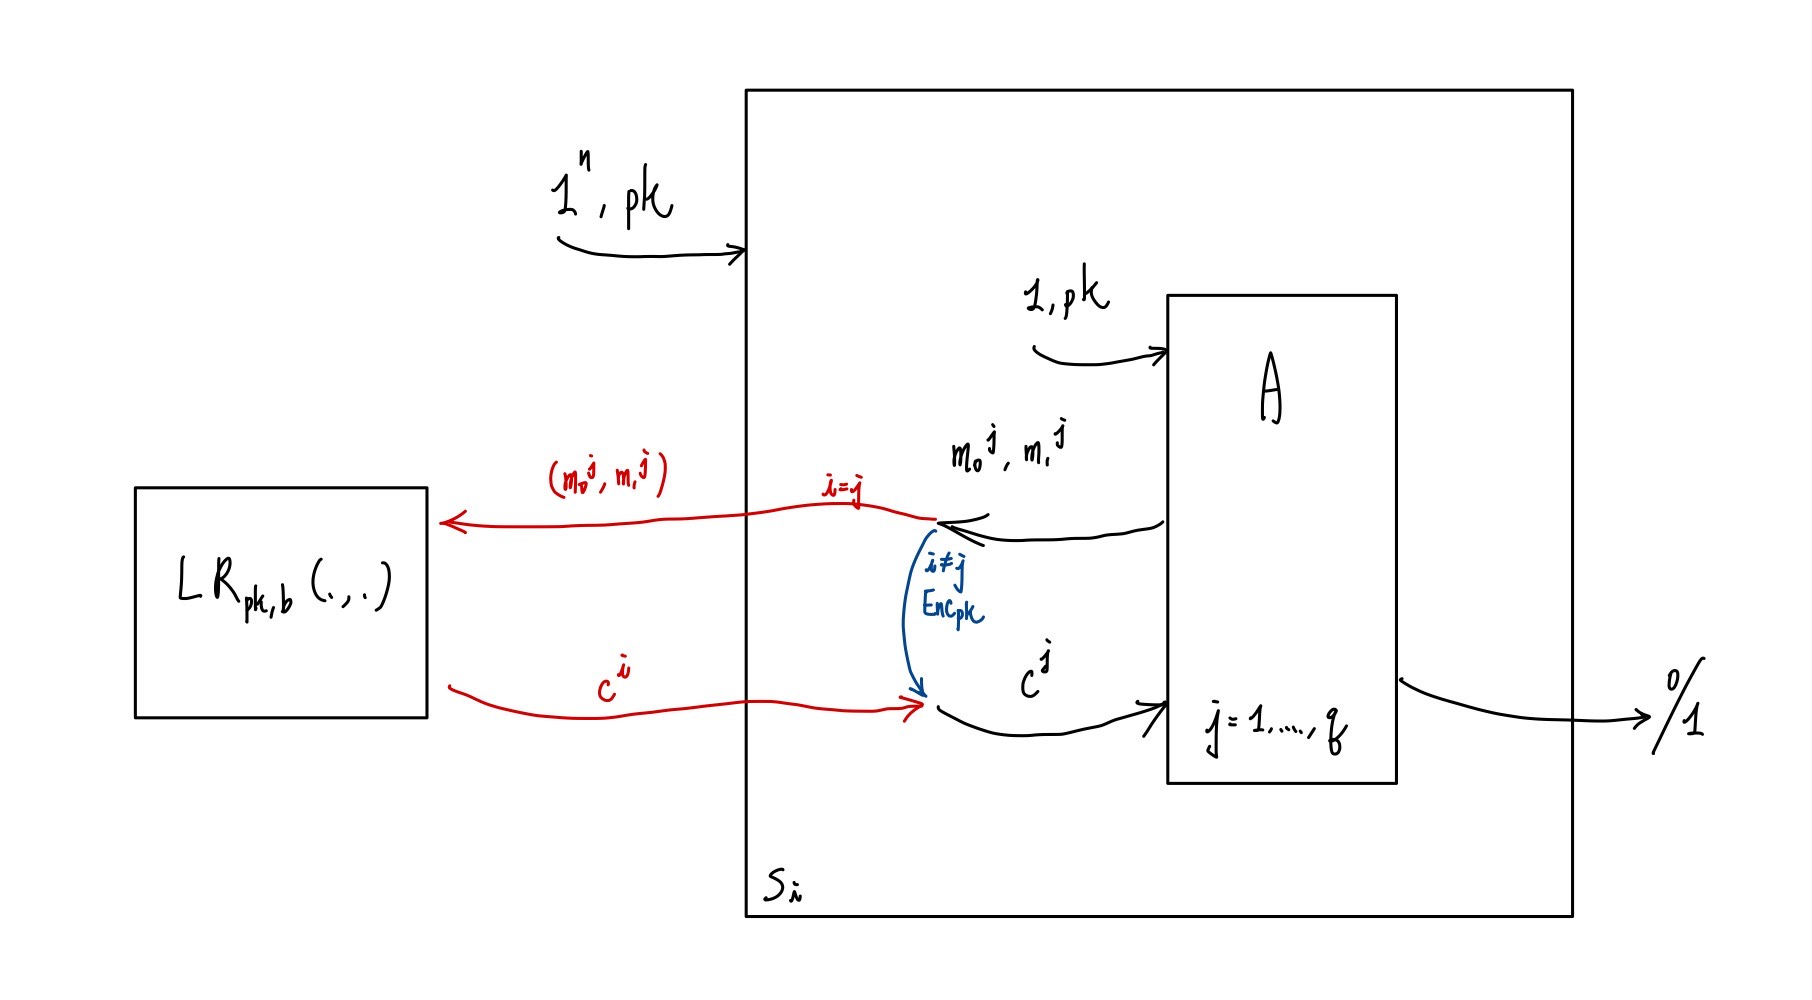
\includegraphics[scale=0.2]{cpa.jpg}
\caption{Simulator Model}
\end{figure}

On $j^{th}$ query of A $(m_0^j,m_1^j)$:
\begin{itemize}
    \item If $j<i$, $S_i$ runs $c \leftarrow Enc_{pk}(m_1^j)$
    \item If $j>i$, $S_i$ runs $c \leftarrow Enc_{pk}(m_0^j)$
    \item If $j=i$, $S_i$ queries its LR oracle and gives the result to $A$
\end{itemize}
\begin{equation}
\begin{cases}
    S_i\text{ is in the left world }(b=0)\text{, then we perfectly simulate }Hybrid(i-1) \\
    S_i\text{ is in the right world }(b=1)\text{, then we perfectly simulate }Hybrid(i)
\end{cases}
\end{equation}
\\
By triangle inequality,
\begin{multline*}
Adv_{\pi}^{CPA}(A) = \big|Pr(A=1\text{ in } Hybrid(0)) - Pr(A=1\text{ in } Hybrid(q)) \big|\\
= \big|Pr(A=1\text{ in } Hybrid(0)) - Pr(A=1\text{ in } Hybrid(1)) + Pr(A=1\text{ in } Hybrid(1)) \\
-Pr(A=1\text{ in } Hybrid(2)) + Pr(A=1\text{ in } Hybrid(2)) \dots -Pr(A=1\text{ in } Hybrid(q)) \big|\\
\le \sum_{i=1}^{q} \underbrace{Adv_{\pi}^{single-CPA}(S_i)}_{negl(n)} = \underbrace{q}_{poly(n)} \cdot negl(n) = negl(n)
\end{multline*}
\\
The theorem implies that we can encrypt long messages bit-by-bit (or block-by-block) or broken up in any other reasonable way. In other words, it is acceptable to convert one call to encryption on long message to many calls to encryption on short messages.
\\
\begin{figure}[H]
    \centering
    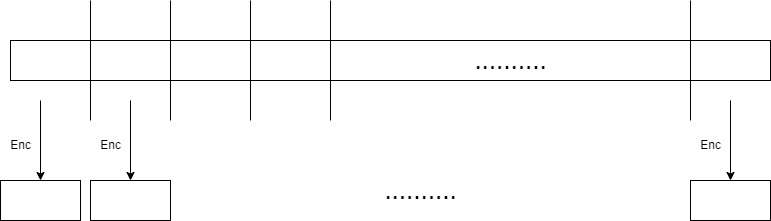
\includegraphics[scale=0.2]{second.jpg}
    \caption{Block-by-block encryption}
\end{figure}

\vspace{5mm}

\noindent \textbf{Theorem}: Any public key encryption scheme with deterministic $Enc_{pk}(.)$ cannot be CPA secure \textbf{even for 1 query}.
\\\\
\textbf{Proof}: query $c \leftarrow LR_{pk,b}(m_0,m_1)$ for any $m_0 \neq m_1$. Then, run $c' = Enc_{pk}(m_0)$. If $c=c'$ outputs 0, else 1. Because the adversary knows the query $(m_0,m_1)$ and the public key $pk$, the adversary has a perfect advantage in distinguishing $c$ and $c'$.

\vspace{10mm}

%=============================================================================
%=============================================================================

\section{El Gamal Cryptosystem}
El Gamal is the public key encryption version of Diffie Hellmen. It works as follows:
$$ Alice \;\autorightleftharpoons{$A=g^a \in G$}{$B=g^b \in G$}\; Bob $$
$$ \text{choose random a }\leftarrow Z_q \;\hspace{3cm}\; \text{choose random }b \leftarrow Z_q $$
$$ K = B^a = g^{ab\text{ mod}q} \in G \;\hspace{3cm}\; K = A^b = g^{ba\text{ mod}q} \in G $$

where $G$ is a group of order $q$ and $g$ is a generator of $G$.
\\\\
$K$  is the secret key derived by two parties. We use the properties of cyclic group to get random number with multiplication.
\\\\
We can look at El Gamal Cryptosystem in terms of $(Gen, Enc, Dec):$
\\
\textbf{Idea}: Basically, message is $M \in G$. The "one-time-pad effect" would involve multiplying $M$ with something random: $K$. 
\begin{itemize} 
    \item $Gen(1^n)$: choose random a $\leftarrow Z_q $ output $(pk=A=g^a \in G, sk=a) \Leftarrow$ what Alice computes
    \item $Enc(pk=A,M \in G)$: choose random $b \leftarrow Z_q$ output ciphertext $(B = g^b \in G, \\C = M \cdot A^b \in G) \Leftarrow $ what Bob computes
    \item $Dec(sk=a,(B,C))$: compute $K=B^a$, output $C \cdot K^{-1} \in G$
\end{itemize}
We need to check the correctness and the security requirement of the cryptosystem.
\\
\\
\textbf{(1) Correctness}: $\forall M \in G$\text{, }$(pk=g^a,sk=a)$
\[Enc(pk,A) = (B = g^b, C = M \cdot (g^a)^b)\]
\[Dec(B,C) = C \cdot (B^a)^{-1} = M \cdot g^{ab} \cdot (g^{(ab)})^{-1} = M\]
\vspace{5mm}
\\
\noindent\textbf{(2) CPA Security}: Based on the DDH assumption over $G: (g,g^a,g^b,g^{ab}) \in G^4$, where $a,b \leftarrow Z_q$, is indistinguishable from $(g,g^a,g^b,g^{c}) \in G^4$, where $a,b,c \leftarrow Z_q$.
\\\\
\textbf{Theorem}: If DDH holds for $G$, then El Gamal is CPA-secure.
\\
\textbf{Proof}: Let $A$ be any feasible p.p.t attacker against El Gamal. Use $A$ to construct the distinguisher against DDH.
\\\\
\begin{figure}[H]
    \centering
    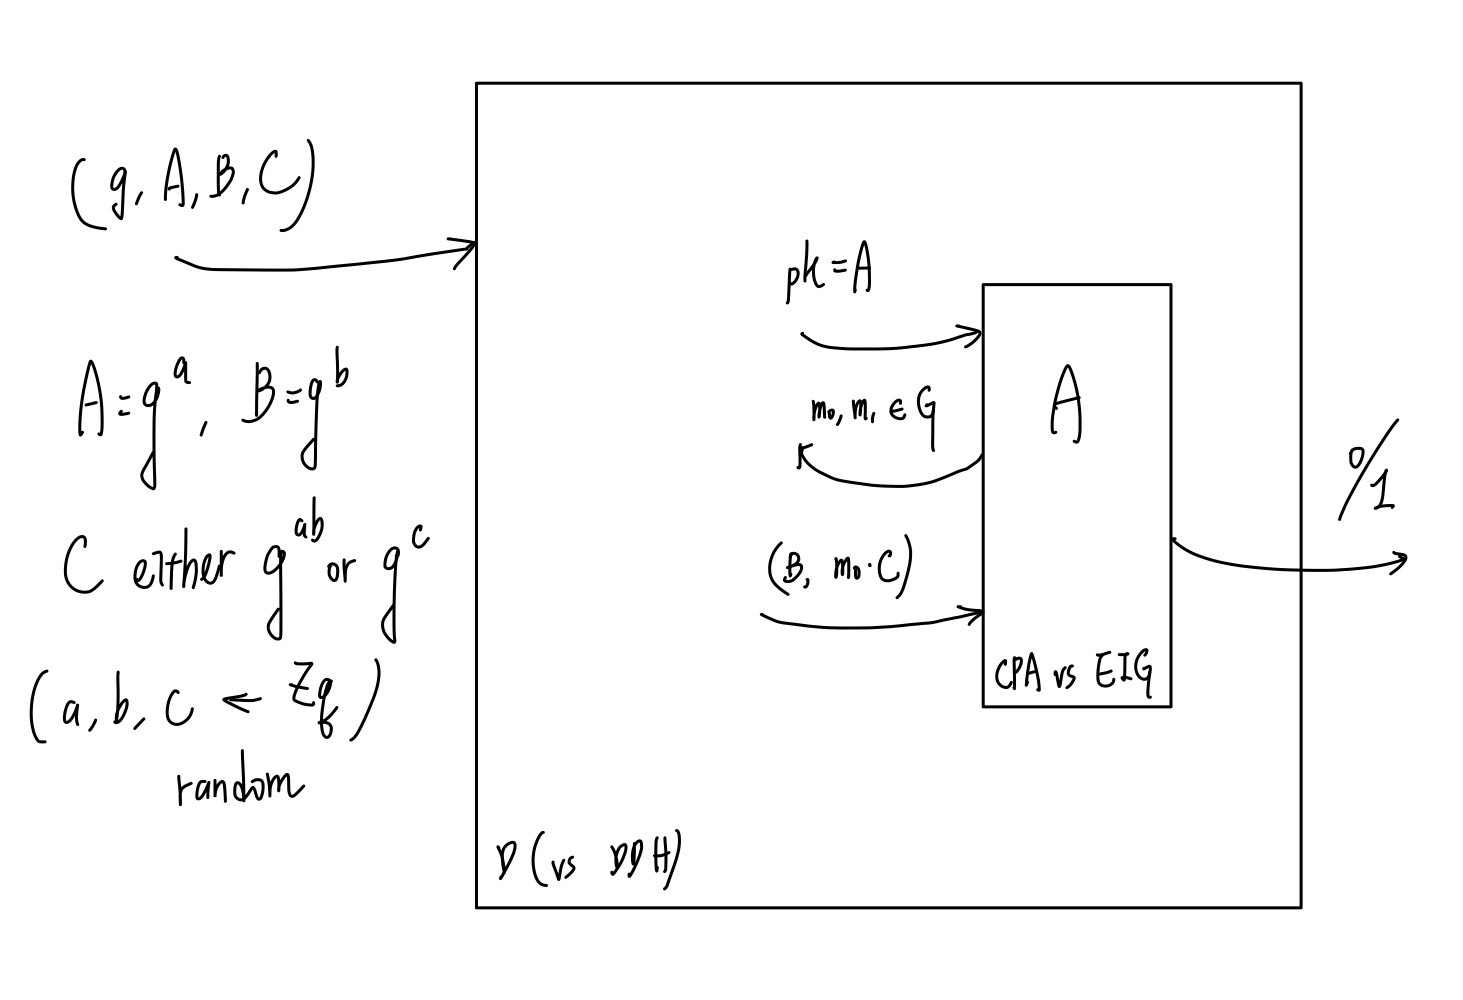
\includegraphics[scale=0.2]{elg.jpg}
    \caption{Use the attacker against El Gamal to construct the distinguisher against DDH}
\end{figure}
\noindent If $(g,A,B,C)$ is a DH tuple ("real world"), D perfectly simulates the left CPA world because $C=g^{ab}$.
\\
Ideal world: $(g,A,B,C)$ is random then $D$ perfectly simulates a "hybrid" CPA world where the ciphertext is two independent random-group elements (regardless of message).
\\
\\
Symmetrically, we can construct $D'$ vs DDH that replies A with $(B,m_1 \cdot C)$
\[Adv^{CPA}(A) \le Adv^{DDH}(D) + Adv^{DDH}(D') = negl(n)+negl(n) = negl(n)\]
\vspace{10mm}

%\lipsum

%=============================================================================
%=============================================================================

\bibliographystyle{alpha}
% Uncomment below if you have any references:
%\bibliography{\jobname}

%=============================================================================
%=============================================================================

\end{document}
